\section{Stream Processing Architecture}\label{sec:concepts}
% Describe different ideas for distribution of events on multiple threads/processing and machines.  


\begin{figure*}[!ht]
    \begin{center}
        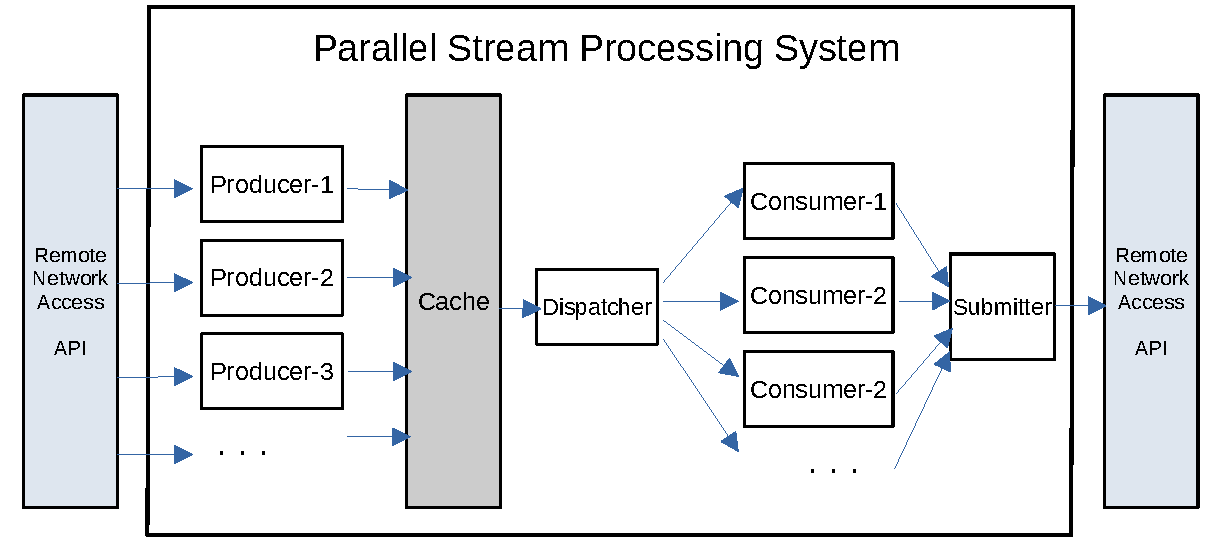
\includegraphics[width=0.8\textwidth]{./images/Parallel-Stream-Processing-System}
        \label{fig:parallel-srream-processing}
        \caption{Distribution of Stream Processing Task using multiple Event Producer and Consumers to process Query 1 and Query 2 }
    \end{center}
\end{figure*}



\section{Implementation Details}\label{sec:implementation}
% Discuss the details of implementation. 



Different data models and serialization have a huge impact on data processing performance \cite{DBLP:conf/cloud/SikdarTJ17}. 



% add code how we do the Query 2. 


\begin{minipage}{0.9\linewidth}
\begin{lstlisting}[caption={Query 2}, label={lst:createDataFrame4},language=Python]
def get_crossover(
    ema_38: float,
    ema_100: float,
    cur_38: float,
    cur_100: float,
    e: ch.Event
) -> Optional[ch.CrossoverEvent]:
""" Helper function for determining crossovers.
Args:
    ema_38 (float): The previous EMA38 value.
    ema_100 (float): The previous EMA100 value.
    cur_38 (float): The current EMA38 value.
    cur_100 (float): The current EMA100 value.
    e (ch.Event): Event.
Returns:
    Optional[ch.Crossover]: A crossover event.
"""
type = None
if ema_38 <= ema_100 and cur_38 > cur_100:
    type = ch.CrossoverEvent.SignalType.Buy
elif ema_38 >= ema_100 and cur_38 < cur_100:
    type = ch.CrossoverEvent.SignalType.Sell

if type is not None and e is not None:
    return ch.CrossoverEvent(
            ts=e.last_trade,
            symbol=e.symbol,
            security_type=e.security_type,
            signal_type=type
        )    
return None
\end{lstlisting}
\end{minipage}





\begin{minipage}{0.9\linewidth}
\begin{lstlisting}[caption={Stream Processing Batch}, label={lst:createDataFrame4},language=Python]
class ProcessBatches (threading.Thread):
""" Producer thread to process batches. """
def __init__(
    self,
    benchmark: Benchmark,
    counter: Counter,
    queue: Queue,
    start_time: int,
    num_consumers: int
) -> None:
    """ Initializes the producer thread.
    Args:
        benchmark (Benchmark): Benchmark to submit to.
        counter (Counter): Counter to synchronize pushing of batches.
        queue (Queue): Queue to push batches to.
        start_time (int): Reference start time.
        num_consumers (int): Number of consumers.
    """
    threading.Thread.__init__(self)
    self.benchmark = benchmark
    self.counter = counter
    self.queue = queue
    self.start_time = start_time
    self.num_consumers = num_consumers        

def run(self):
    """ Processes batches by pushing onto the queue. """

    while self.benchmark.has_next():
        batch = self.benchmark.next()
        obj = split_batch(batch, self.num_consumers, self.start_time)
        
        # wait for counter to equal batch num 
        while not self.counter.is_value(obj[2]):
            pass

        # at this point counter == batch_num
        self.queue.put(obj, block=True)

        # increment counter so next batch can be put into the queue
        self.counter.increment()
\end{lstlisting}
\end{minipage}
    
    


